

%=================================================================
% Outline
%=================================================================
%\section{Introduction}
%\input{outline_currentsection}
\section*{Outline}% Make it easy to jump to this page in the PDF

% Auto-generate the TOC slide(s)
\begin{frame}
  \frametitle{Outline}
  %\tableofcontents[currentsection]
  \tableofcontents
\end{frame}




\section{\libMesh{} History and Goals}
%%%%%%%%%%%%%%%%%%%%%%%%%%%%%%%%%%%%%%%%%%%%%%%%%
\frame
{
  \frametitle{History}

  \begin{center}
  \includegraphics[width=.3\textwidth]{cfdlab}
  \end{center}

  \begin{itemize}
    \item CFDLab, University of Texas at Austin
      \begin{itemize}
        \item Computational Fluid Dynamics research, from creeping
          (Roy Stogner) to incompressible (John Peterson) to hypersonic
          (Benjamin Kirk)
        \item Adaptive Finite Element Method research (Dr. Graham F.\ Carey)
        \item High-performance computing research (Bill Barth)
        \item Software engineering experience (Robert McLay)
        \item<3-> Stubbornness (Benjamin Kirk, John Peterson, Roy Stogner, ...)
      \end{itemize}
    \item<2-> ``No one ever got a PhD from here for writing a code.'' - Dr. Graham F.\ Carey
  \end{itemize}  


}



%%%%%%%%%%%%%%%%%%%%%%%%%%%%%%%%%%%%%%%%%%%%%%%%%
\frame
{
  \begin{center}
  \includegraphics[width=.3\textwidth]{cfdlab}
  \end{center}

  \begin{block}{The standard Ph.D.-candidate software development
    process:}
  \pause
  \begin{itemize}[<+->]
    \item Create pseudocode
      \begin{itemize}[<+->]
        \item (throw it away; it won't match the real code you
          end up writing)
      \end{itemize}
    \item Create Matlab prototypes, fast
      \begin{itemize}[<+->]
        \item You're just solving one problem
        \item Don't waste time on
          documentation for slow-witted users
        \item You're just going to rewrite the bad hacks
          anyway
      \end{itemize}
    \item Rewrite from scratch (maybe in Fortran?)
      \begin{itemize}[<+->]
        \item ``the single worst strategic mistake'' - Joel Spolsky, 2000
        \item ``Other slow-witted users'' includes ``myself, 2 years
          later''
        \item Bad hacks may now be load-bearing dependencies
      \end{itemize}
    \item Graduate, throw it all away, go work on a ``real'' code
  \end{itemize}  
  \end{block}


}


 

%%%%%%%%%%%%%%%%%%%%%%%%%%%%%%%%%%%%%%%%%%%%%%%%%
\frame
{
  \begin{center}
  \includegraphics[width=.3\textwidth]{cfdlab}
  \end{center}

  \begin{block}{libMesh Development Ingredients}
  \pause
  \begin{itemize}[<+->]
    \item Inspiration (Wolfgang Bangerth + deal.II, Robert McLay + MGFLO)
    \item Genius (Ben Kirk, John Peterson, 2002)
    \item Collaboration (Daniel Dreyer, Steffen Petersen, 2003; Roy
      Stogner 2004; David Knezevic 2005; Derek Gaston 2006)
    \item Flexibility
      \begin{itemize}[<+->]
        \item Documentation: teaching is the best way to learn
        \item Abstraction: purpose first, algorithm second, data third
          \begin{itemize}[<+->]
            \item C++: OOP \emph{and} ``only pay for what you use''
          \end{itemize}
        \item Encapsulation: only promise what you can guarantee
        \item Modularity: only use what you must demand
        \item Testing: don't break what you promise
      \end{itemize}
  \end{itemize}  
  \end{block}


}


 




%%%%%%%%%%%%%%%%%%%%%%%%%%%%%%%%%%%%%%%%%%%%%%%%%
\frame
{
  \frametitle{The \libMesh{} Software Library}
  \begin{itemize}
    \item In 2002, the \libMesh{} library was created with these ideas
      and concerns in mind.
    \item Primary goal is to provide individual tools: data structures
      and algorithms that can be shared by widely differing physical
      applications, that may need some combination of
      \begin{itemize}
      \item Implicit numerical methods
      \item Adaptive mesh refinement techniques
      \item Parallel computing 
      \end{itemize}
    \item Unifying theme: \emphcolor{mesh-based simulation of partial differential equations (PDEs)}.
      \begin{itemize}
      \item Continuous and discontinuous Finite Element Methods
      \item Finite Volume Methods
      \item Even many ``mesh-free'' methods
      \end{itemize}
  \end{itemize}
}




 

%%%%%%%%%%%%%%%%%%%%%%%%%%%%%%%%%%%%%%%%%%%%%%%%%
\frame
{
  \frametitle{The \libMesh{} Software Library}

  \begin{block}{A Toolkit, not a Framework}
    \begin{itemize}
      \item \libMesh{} was designed to give students, researchers,
        scientists, and engineers tools to \emphcolor{develop
        simulation codes} or \emphcolor{rapidly implement a numerical
        method}.
      \item \libMesh{} is not an application.
      \item It does not ``solve problem XYZ.''
        \begin{itemize}
          \item It was designed to help \cancel{users} researchers
            create their own application to solve problem XYZ,
            quickly, with advanced numerical algorithms on
            high-performance computing platforms.
          \item It has since been used to create professional
            application frameworks to solve many problems, combined,
            with user-friendly interfaces.
        \end{itemize}
    \end{itemize}    
  \end{block}
} 


%%%%%%%%%%%%%%%%%%%%%%%%%%%%%%%%%%%%%%%%%%%%%%%%%
\frame
{
  \frametitle{Software Reuse}
  \begin{itemize}
    \item When \libMesh{} was created in 2002, many high-quality
      software libraries implemented some fraction of the end-to-end PDE simulation process:
      \begin{itemize}
        \item Linear algebra (Laspack, PETSc)
        \item Partitioning algorithms for domain decomposition
        \item Visualization of solution files
        \item \ldots
      \end{itemize}
    \item \libMesh{} tries to provide flexible, extensible, abstract interfaces to existing software when possible.
    \item We implemented ``glue'' to these pieces, plus what was missing at the time:
      \begin{itemize}
        \item \emphcolor{Flexible data structures for discretizating of spatial domains and systems of PDEs posed on them.}
      \end{itemize}          
  \end{itemize}  
}




\begin{frame}{libMesh Community}
\begin{columns}
\column{.4\textwidth}
\begin{block}{Scope}
\begin{itemize}
\item Free, Open source
\begin{itemize}
\item LGPL2 for core
\end{itemize}
\item 153 Ph.D.\ theses from users, 2254 papers (240+ in 2024)
\item 15 contributors in 2024, 102 historically
\end{itemize}
\end{block}

\column{.6\textwidth}
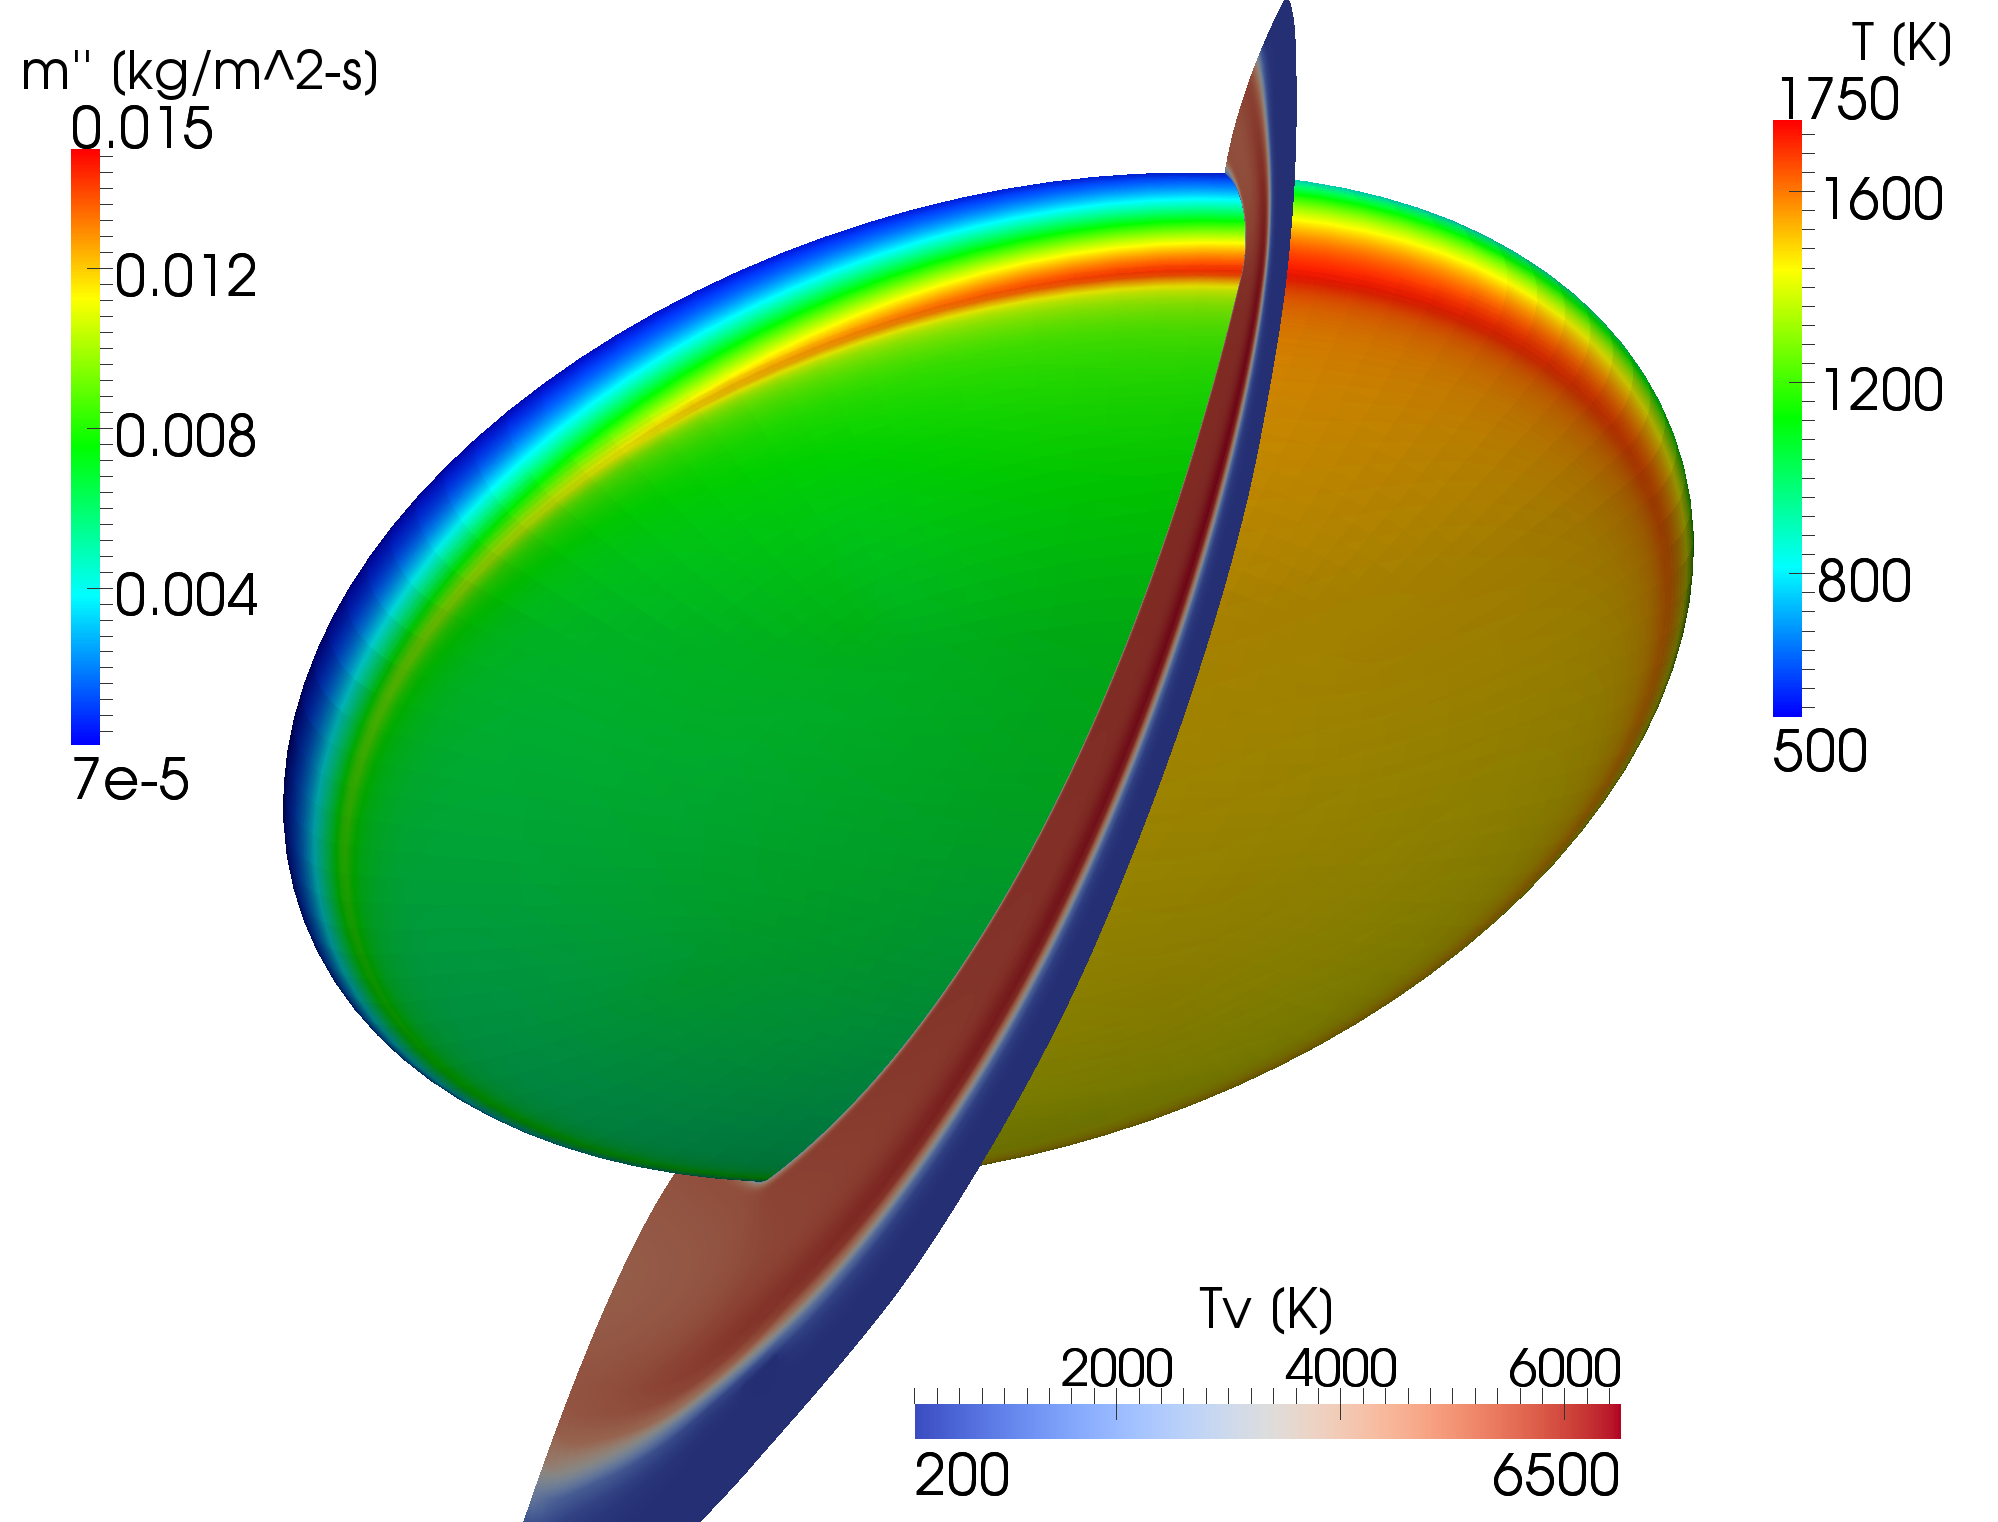
\includegraphics[width=.45\textwidth]{ablating_hs_wbg}
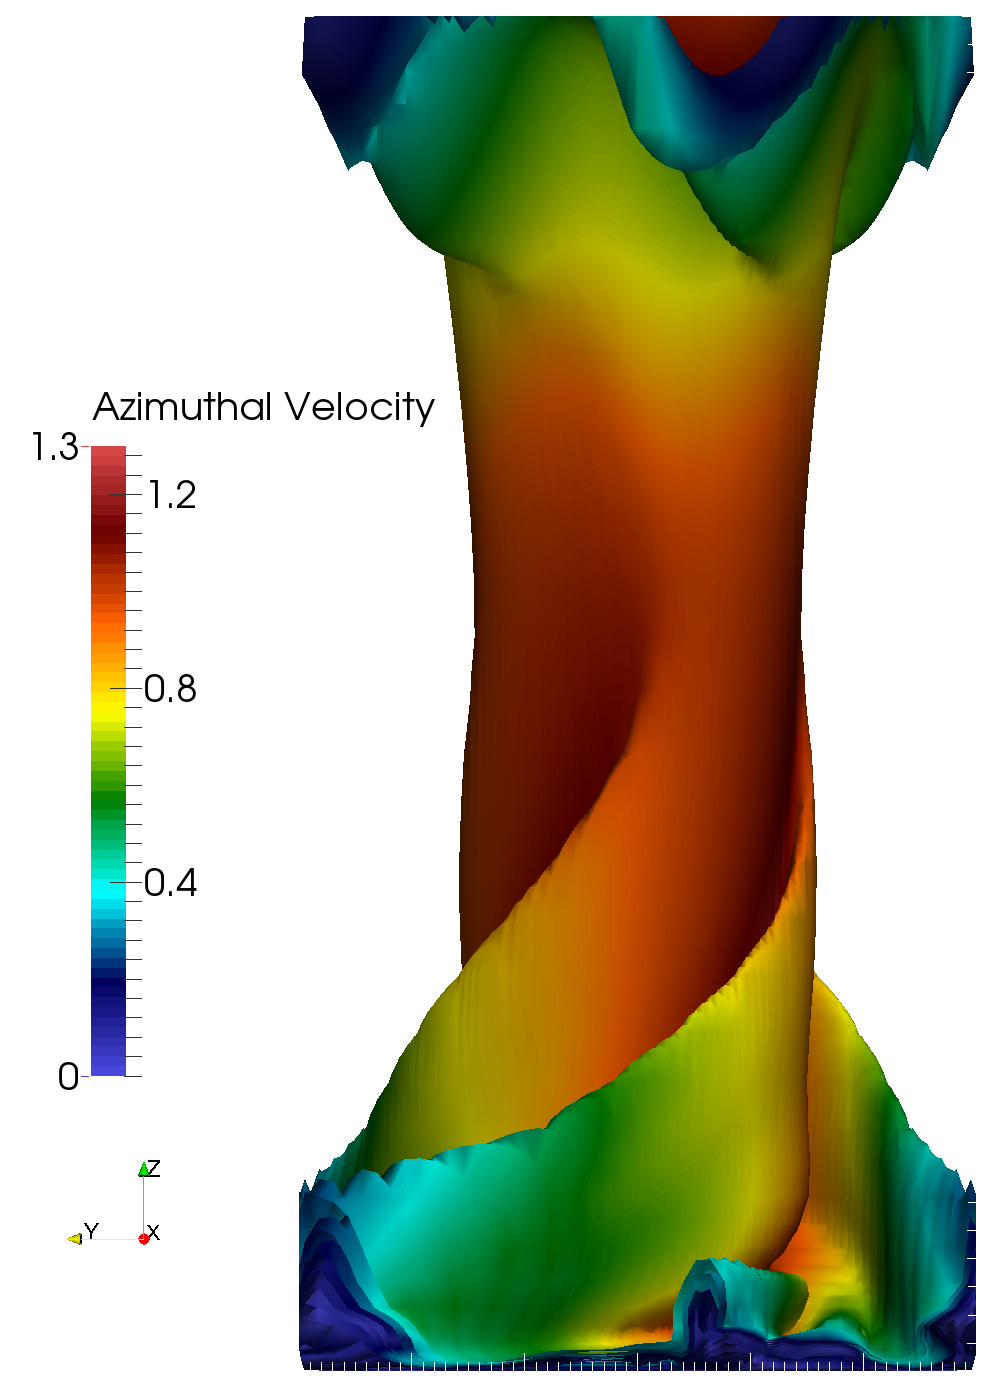
\includegraphics[width=.25\textwidth]{sov}
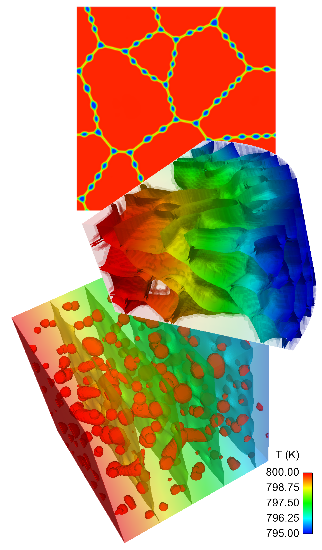
\includegraphics[width=.25\textwidth]{marmot1b}
\end{columns}

\begin{columns}
\column{.35\textwidth}
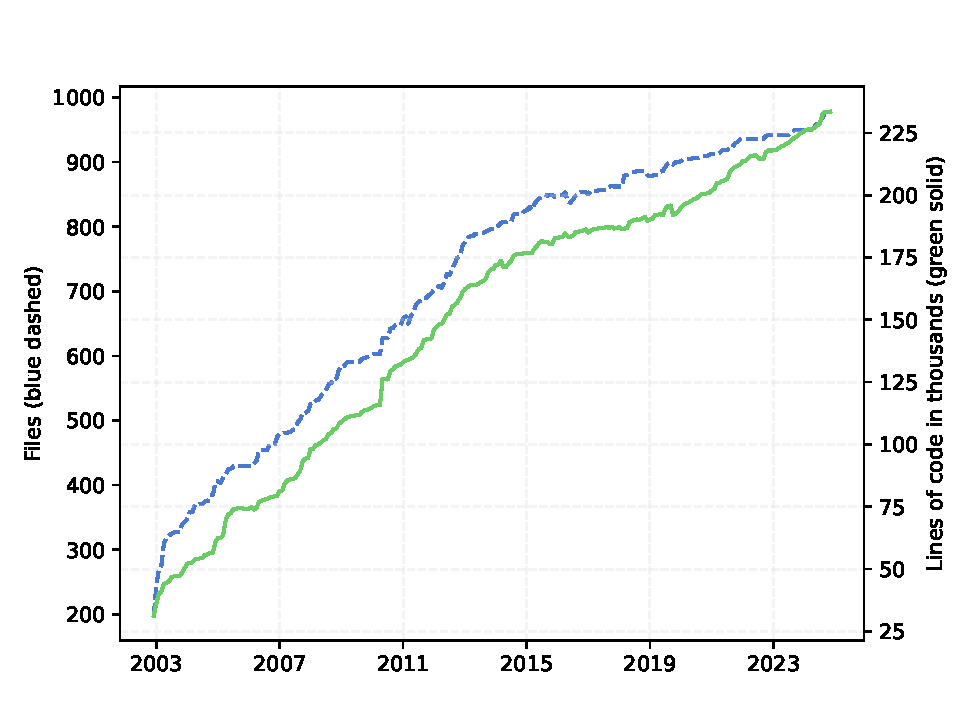
\includegraphics[width=\textwidth]{cloc_libmesh}

\column{.65\textwidth}
\begin{block}{Challenges}
\begin{itemize}
\item Radically different application types
\item Widely dispersed core developers
\begin{itemize}
\item At peak: INL, UT-Austin, U.Buffalo, JSC, MIT, Harvard, Argonne
\end{itemize}
\item OSS, commercial, private applications
\end{itemize}
\end{block}
\end{columns}

\end{frame}


\begin{frame}[t]
  \begin{columns}
    \column{.6\textwidth}
    \begin{center}
      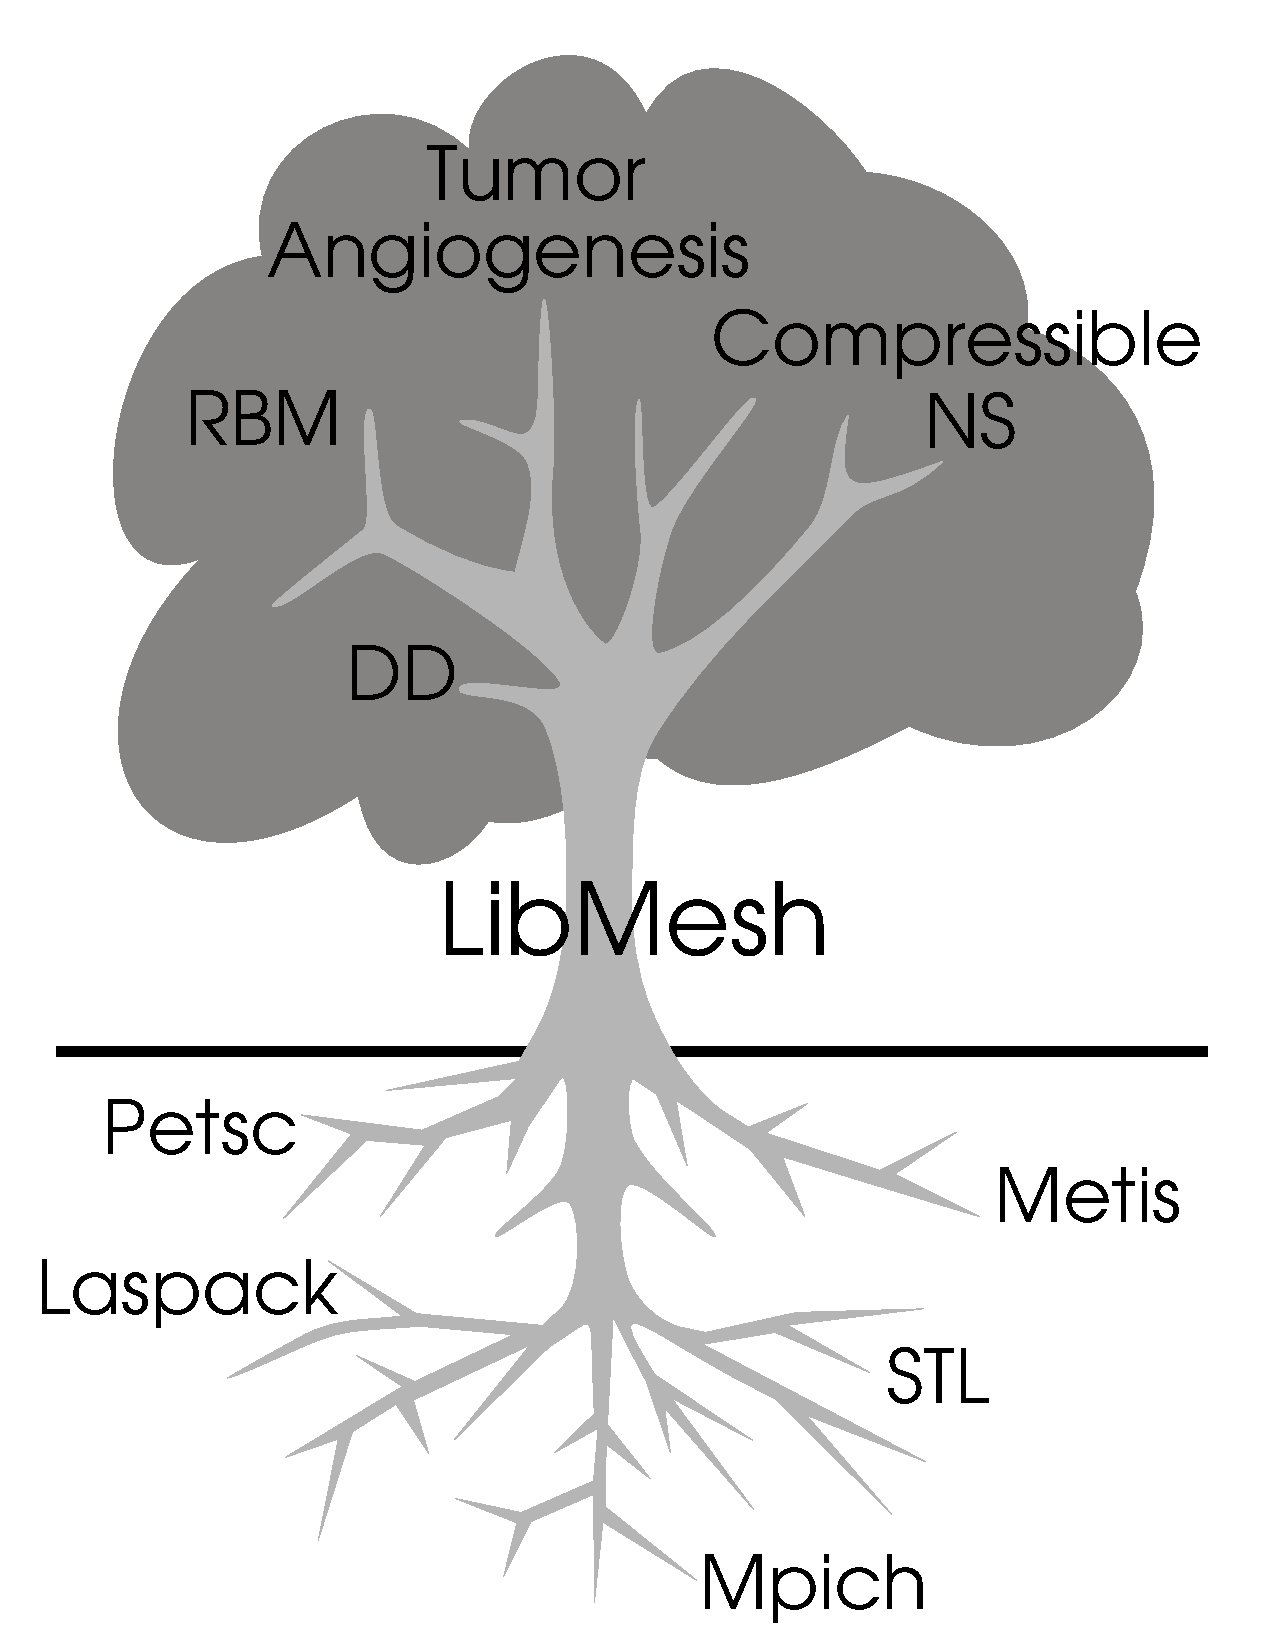
\includegraphics[width=.9\textwidth]{mytreeandroots_allnames}
    \end{center}
    \column{.35\textwidth}
    \begin{itemize}
      \item Foundational (typically optional) library access via LibMesh's ``roots''.
      \item Application ``branches'' built off the library ``trunk''.
      \item Additional middleware layers (e.g. Akselos, GRINS, MOOSE) for more complex applications
    \end{itemize}
  \end{columns}

\end{frame}
